\documentclass{beamer}
\usepackage[utf8]{inputenc}
\usepackage{graphicx}
\usepackage{listings}

\usepackage{xcolor}

\lstdefinestyle{base}{
	language=C++,
	emptylines=1,
	breaklines=true,
	basicstyle=\ttfamily\color{black},
	moredelim=**[is][\bf\color{red}]{@}{@},
}

\usetheme[]{boxes}
\usecolortheme{seagull}

%\usepackage{french}
\title{Modèles et techniques en programmation parallèle hybride et multi-c\oe urs}
\subtitle{Introduction au parall\'elisme multithreads}
\author{Marc Tajchman}\institute{CEA - DEN/DM2S/STMF/LMES}
\date{10/08/2020}

\begin{document}
\begin{frame}
	\titlepage
\end{frame}

\large
\begin{frame}
	\section{Parallélisme multi-threads en mémoire partagée}
	\frametitle{Parallélisme multi-threads en mémoire partagée}
	
	\vfill
	Le but du parallélisme multithreads est de découper l'ensemble des instructions en plusieurs parties et d'exécuter (le plus possible) simultanément ces différentes parties par des threads (exécutions) sur des c\oe urs différents.
	
	
	\vfill
	On appellera la version du code non parallélisé : ``séquentiel''.
	
	\vfill
    Dans le cas le plus simple, le nombre de threads est égal au nombre de c\oe urs.

	\vfill
	En mémoire partagée signifie que différents groupes d'instructions travaillent sur des données contenues dans la même mémoire. Il faut donc faire attention que les modifications faites par certaines instructions ne perturbent pas les données utilisées par d'autres instructions.
	\vfill
	
\end{frame}

\large
\begin{frame}[fragile]
	Exemple 1: si \verb|u| et \verb|v| sont des vecteurs de taille \verb|n > 4|, on veut calculer la boucle {\tt for}:
	
	\begin{equation}
	\begin{array}{l}
for (i=1; i<n-1; i++) \\
\quad  v_i = (u_{i-1} + 2*u_{i} + u_{i+1})/4;
\end{array}
	\end{equation}
	
	\vfill
	Ces instructions (pour différentes valeurs de $i$) utilisent des composantes de \verb|u| différentes, mais (presque) toutes les composantes de $u$ sont utilisées par plusieurs instructions de la boucle {\tt for}.
	
	\vfill
	\textcolor{blue}{Les composantes de u ne sont pas modifiées par les instructions.}
	
	\vfill
	\textcolor{blue}{Les composantes de v sont modifiées (mais chaque instruction calcule une composante différente).}
	
	\vfill
	On remarque que le calcul de $v_i$ ne dépend pas de celui de $v_j$ ($j \neq i$) et donc ces 2 calculs peuvent se faire en même temps par 2 ex\'ecutions différentes qui utilisent les mêmes vecteurs u et v.
		
\end{frame}

\begin{frame}
	\parbox[t][1cm]{10cm}{1. Avant d'exécuter les 2 instructions (i=2 et i=3) :}
   \begin{center}
   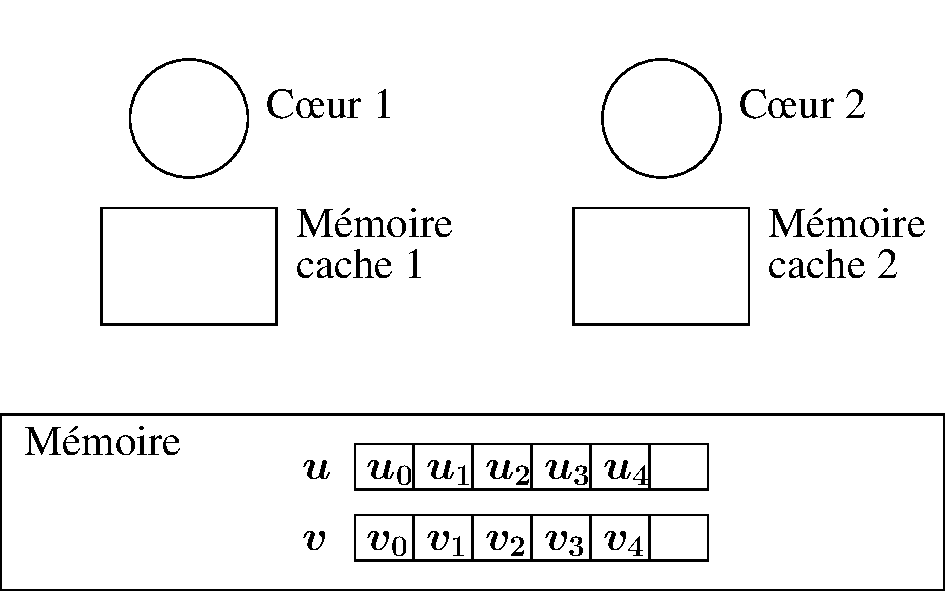
\includegraphics[scale=0.6]{../../Images/multithread0}
   \end{center}
\end{frame}

\begin{frame}
	\parbox[t][1cm]{10cm}{2. Les composantes de $u$ sont recopiées dans les mémoires cache :}
   \begin{center}
	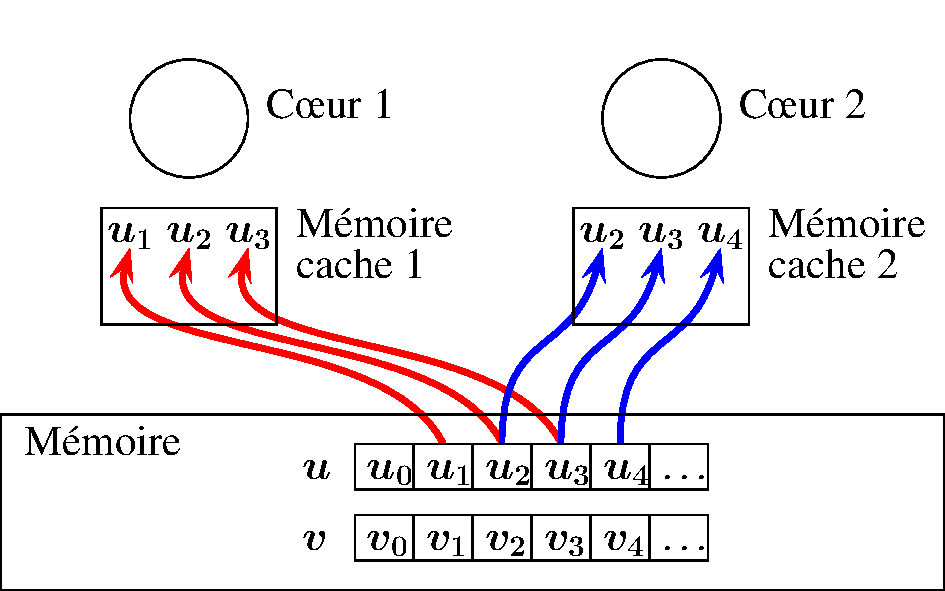
\includegraphics[scale=0.6]{../../Images/multithread1}
   \end{center}
\end{frame}

\begin{frame}
	\parbox[t][1cm]{10cm}{3. Les composantes de $u$ sont recopiées dans les mémoires internes des processeurs:}
   \begin{center}
	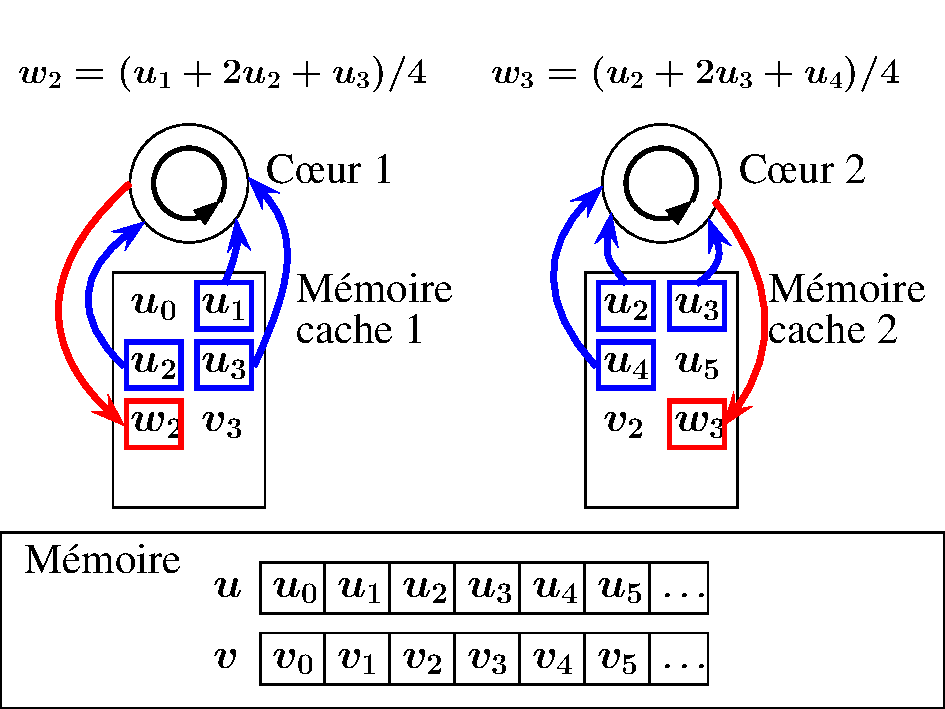
\includegraphics[scale=0.6]{../../Images/multithread2}
   \end{center}
\end{frame}

\begin{frame}
	\parbox[t][1cm]{10cm}{4. Le calcul est effectué dans les c\oe urs (2 instructions en //) :
	}
   \begin{center}
	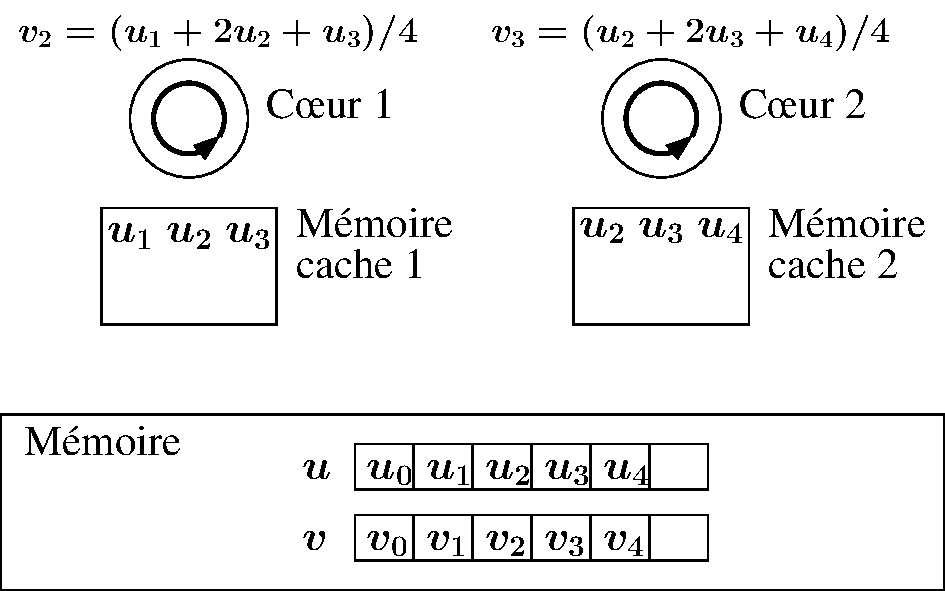
\includegraphics[scale=0.6]{../../Images/multithread3}
   \end{center}
\end{frame}

\begin{frame}
	\parbox[t][1cm]{10cm}{5. Le résultat est recopié dans la mémoire cache :}
	\begin{center} 
		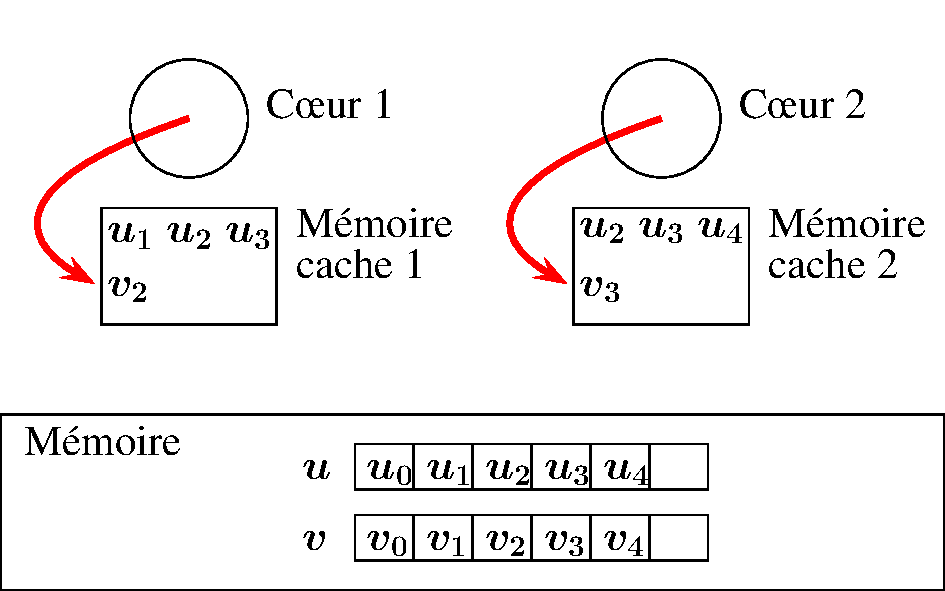
\includegraphics[scale=0.6]{../../Images/multithread4}
	\end{center}
\end{frame}

\begin{frame}
	\parbox[t][1cm]{10cm}{6. Le résultat est recopié dans la mémoire principale :}
	\begin{center}
		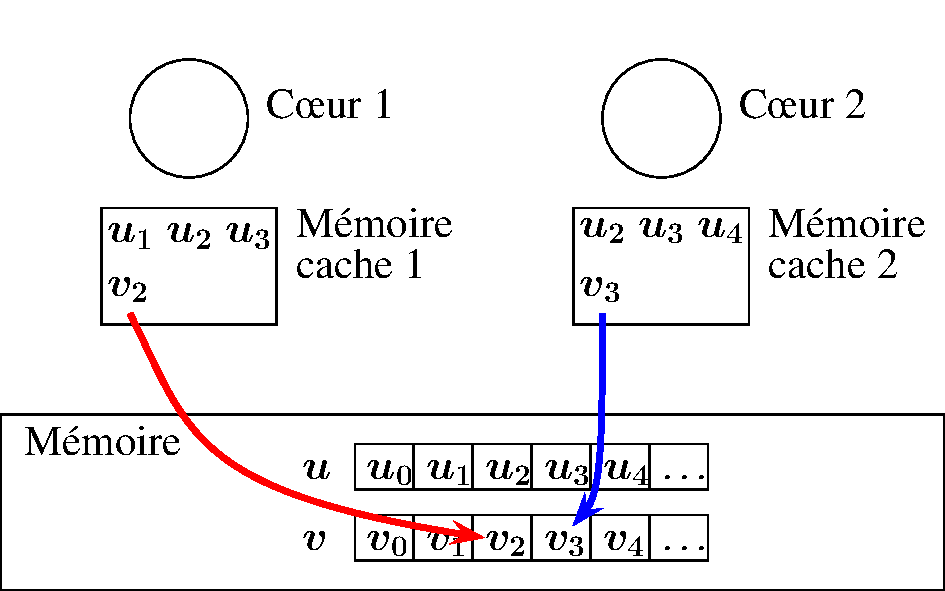
\includegraphics[scale=0.6]{../../Images/multithread5}
	\end{center}
\end{frame}

\begin{frame}[fragile]
	Le plus simple est de découper la boucle séquentielle :
	
	\begin{lstlisting}
for (i=1; i<n-1; i++)
   v[i] = (u[i-1] + 2*u[i] + u[i+1])/4;
	\end{lstlisting}
	
\vfill
	en $K$ sous-boucles :
	
\begin{lstlisting}
for (i=p[k]; i<p[k+1]; i++)    // k = 0...K-1
   v[i] = (u[i-1] + 2*u[i] + u[i+1])/4;
\end{lstlisting}

avec {\tt p[0] = 1} et {\tt p[K] = n-1}

\vfill
L'exécution de toutes les sous-boucles est identique à l'exécution de la boucle complète.
Toutes les sous-boucles doivent si possible être exécutées en même temps.
\end{frame}


\begin{frame}[fragile]
	\vfill
	Le principal (mais pas le seul) outil pour coder du parallélisme multithreads est OpenMP.
	
	\vfill
	On ajoute une ligne avant la boucle (pragma)

\lstset{%
	language={C++},
	breaklines=true,
	captionpos=b,
	basicstyle=\ttfamily,
	moredelim=[il][\color{red}]{/+},%
}

\begin{center}
\begin{lstlisting}{C++}
/+#pragma omp parallel for
for (i=1; i<n-1; i++)
  v[i] = (u[i-1] + 2*u[i] + u[i+1])/4;
\end{lstlisting}
\end{center}

\begin{itemize}
	\item la ligne qui commence par \verb|#pragma| est appelée pragma
	\item en fonction des options de compilation, cette ligne est ignorée ou pas
    \item le compilateur va découper lui-même la boucle en sous-boucles en répartissant les sous-boucles entre les threads
\end{itemize}

\end{frame}

\begin{frame}

Avantages:
\begin{itemize}
	\item un seul code source pour les versions parallèle ou séquentiel
	\item on peut choisir les boucles qu'on veut paralléliser ou non (parallélisation incrémentale)
	\item facile à coder
\end{itemize}
\vfill

Désavantages et difficultés:
\begin{itemize}
	\item les performances sont parfois décevantes
	\item attention aux variables partagées par différentes itérations d'une boucle
	\item pas beaucoup de contrôle sur le placement des threads et sur le découpage en sous-boucles
\end{itemize}

\end{frame}

\begin{frame}[fragile]

Pour compiler du code utilisant OpenMP, on utilise une option de compilation (qui dépend du compilateur : -fopenmp pour gcc/g++/gfortran).

\vfill
Pour exécuter un code utilisant plusieurs threads, il y a plusieurs possibilités:
\begin{itemize}
	\item définir une variable d'environnement \verb|OMP_NUM_THREADS|, par exemple :
	\begin{lstlisting}
	OMP_NUM_THREADS=5 ./code.exe
	\end{lstlisting}
	\item appeler dans le code source la fonction 
	\begin{lstlisting}
	omp_set_num_threads(5);
	\end{lstlisting}
\end{itemize}
\vfill
\end{frame}

\begin{frame}
	Exemple OpenMP 1
\end{frame}

\lstset{%
	language={C++},
	breaklines=true,
	numbers=left,
	numberstyle=\footnotesize,
	captionpos=b,
	basicstyle=\ttfamily,
	keywordstyle=\bfseries\color{blue},
	commentstyle=\itshape\color{green},
	moredelim=[il][\color{red}]{/+},%
}

\begin{frame}[fragile]
	Source C++ séquentiel:
{
	\normalsize
	\lstinputlisting{Exemples/Exemple1/main.cxx}	
}	
\end{frame}


\end{document}